
\section{III - Descente de gradient}
\begin{frame}{III - Descente de gradient}
    \begin{block}{Descente de gradient}
        La Descente de Gradient est un algorithme d’optimisation qui permet de trouver un minimum local d'une fonction en convergeant progressivement. \\
        Dans l'apprentissage des réseaux de neurones, la descente de gradient est utilisée pour trouver le minimum d'une fonction "coût", évaluant l'erreur entre la valeur de sortie du réseau et celle attendue. \\
        Cette fonction d'erreur est noté $f : s \mapsto (s - s_{attendue})^2$, avec $s$ la sortie donnée par le modèle et $s_{attendue}$ la sortie cible. \\
        En effet, trouver des paramètres (poids, architecture du réseau, fonction d'activation) permettant d'avoir une erreur nulle revient à résoudre le problème qu'évalue cette fonction coût par rapport aux données d'entrée.
    \end{block}
\end{frame}

\begin{frame}{III - Descente de gradient}
    \begin{block}{Algorithme du gradient}
        Soit $n \in \mathbb{N}, \varepsilon > 0$. On munit $\mathbb{R}^n$ de son produit scalaire canonique. \\
        Soit $f$ une fonction différentiable de $\mathbb{R}^n \to \mathbb{R}$. \\
        Soit $x_0$ une valeur initiale aléatoire, $t$ le taux d'apprentissage. \\
        Supposons $x_0, \ldots, x_k$ construits. \\
        • Si $\norme{\nabla f(x_k)} \leq \varepsilon$, on s'arrête. \\
        • Sinon on pose $x_{k+1} = x_k - t \nabla f(x_k)$ \\
    \end{block}
    
    \begin{figure}
        \centering
        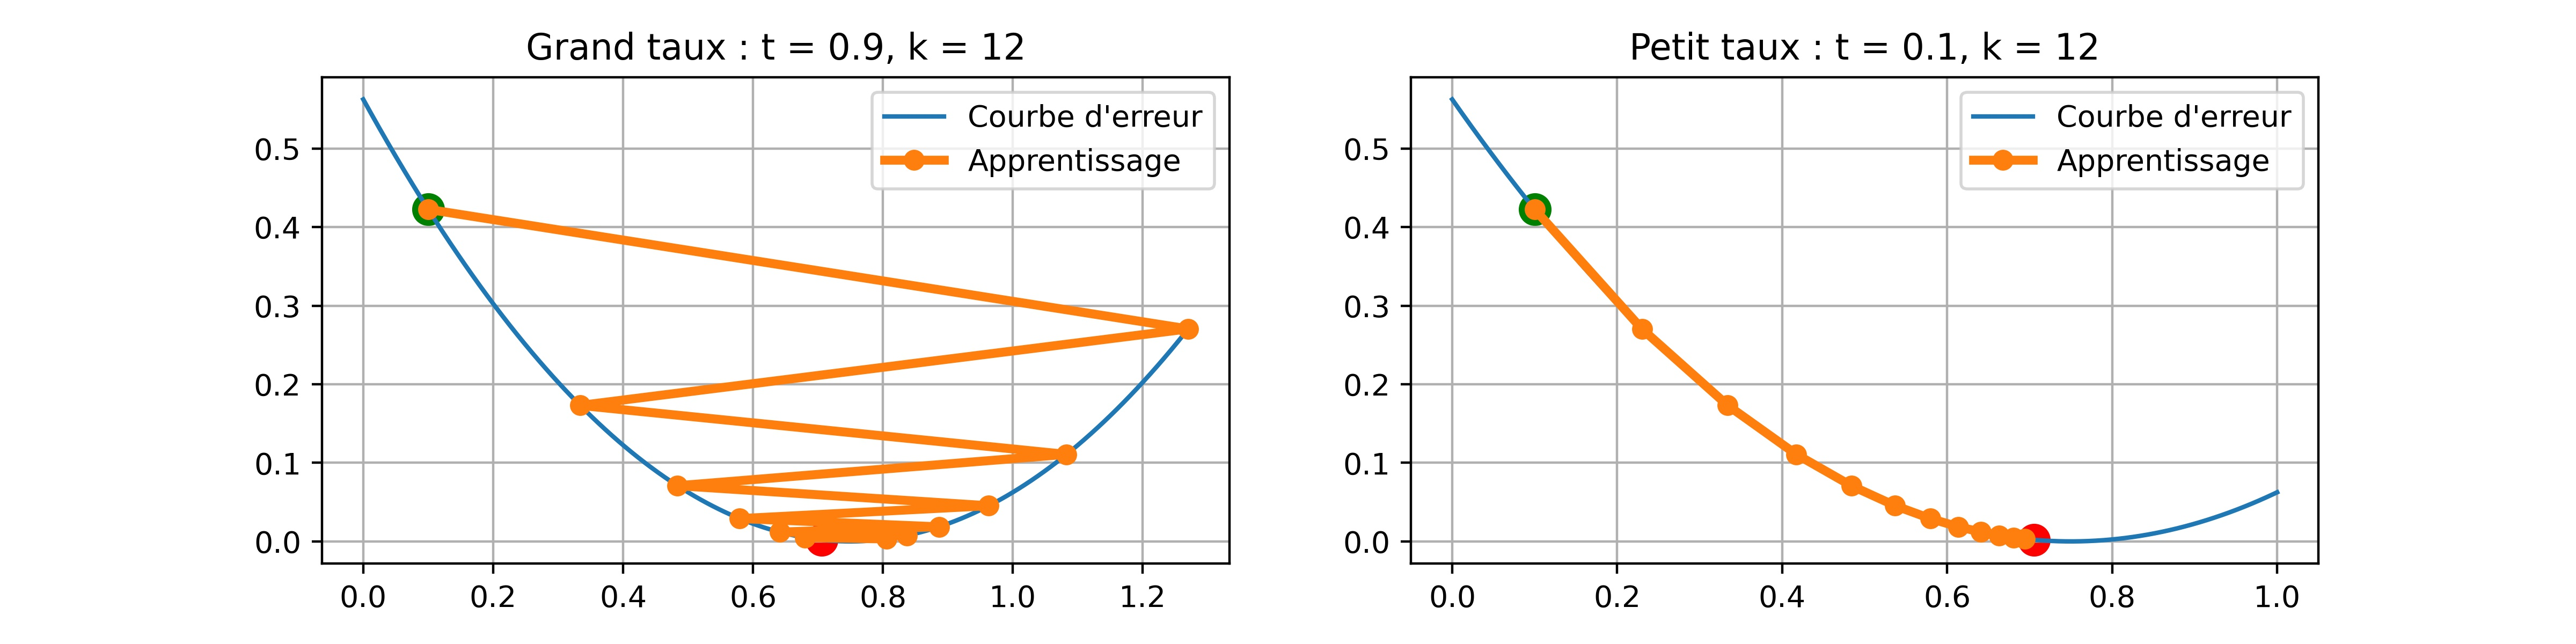
\includegraphics[height=75px]{1-DescenteGradient.jpg}
        \caption{Descente de Gradient pour $f(x) = (x-0.75)^2$; $x_0=0.1$ et $\varepsilon = 0.1$}
    \end{figure}
\end{frame}

\begin{frame}{III - Importance du choix du taux d'apprentissage}
    Pour la suite on continuera avec la fonction $f(x) = (x-0.75)^2$ et $x_0=0.1$. \\
    On montre qu'en choisissant un taux d'apprentissage trop petit ou trop grand, il est possible que la descente de gradient diverge, ou ne converge pas assez vite.
    \begin{figure}
        \centering
        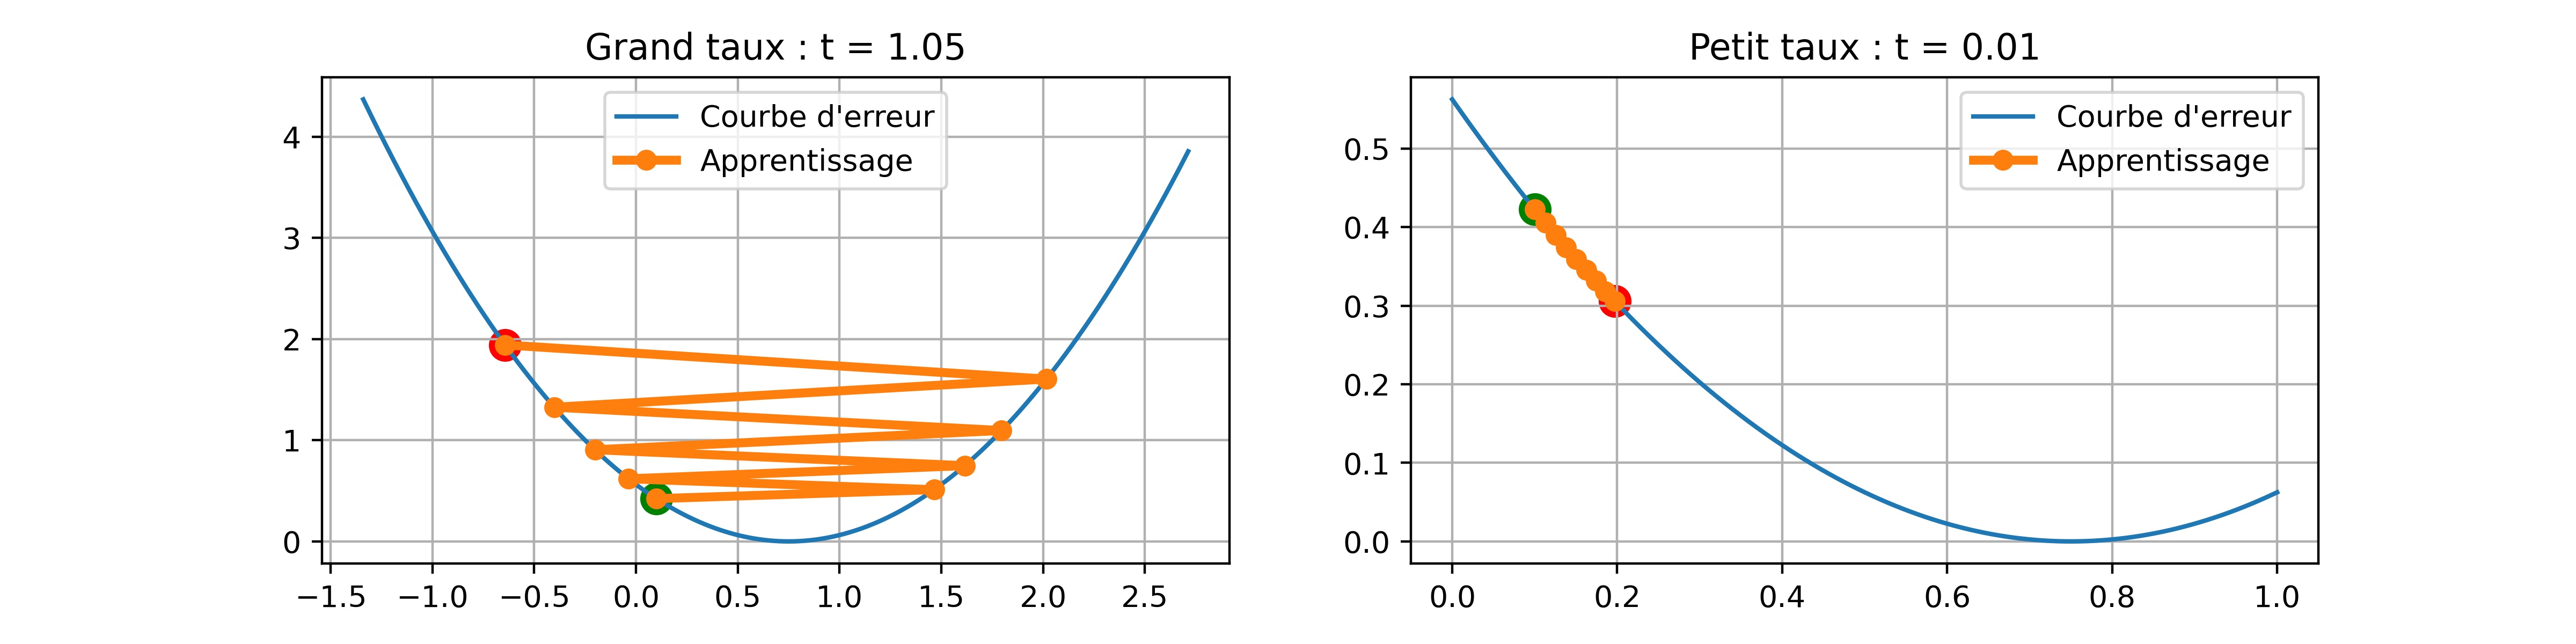
\includegraphics[height=80px]{2-DescenteGradient.jpg}
        \caption{Descente de Gradient on force l'arrêt à $k=8$}
    \end{figure}
\end{frame}

\begin{frame}{III - Utilisation du Moment}
    \begin{block}{III - Descente de gradient avec moment}
        $x_0$ aléatoire et le moment $\omega_0 = 0$.
        Supposons $x_0, \ldots, x_k$ et $\omega_0, \ldots, \omega_k$ construits. \\
        • On pose $\omega_{k+1} = \gamma \omega_k + t \nabla f(x_k)$ \\
        • On pose $x_{k+1} = x_k - \omega_{k+1}$
    \end{block}
    \begin{figure}
        \centering
        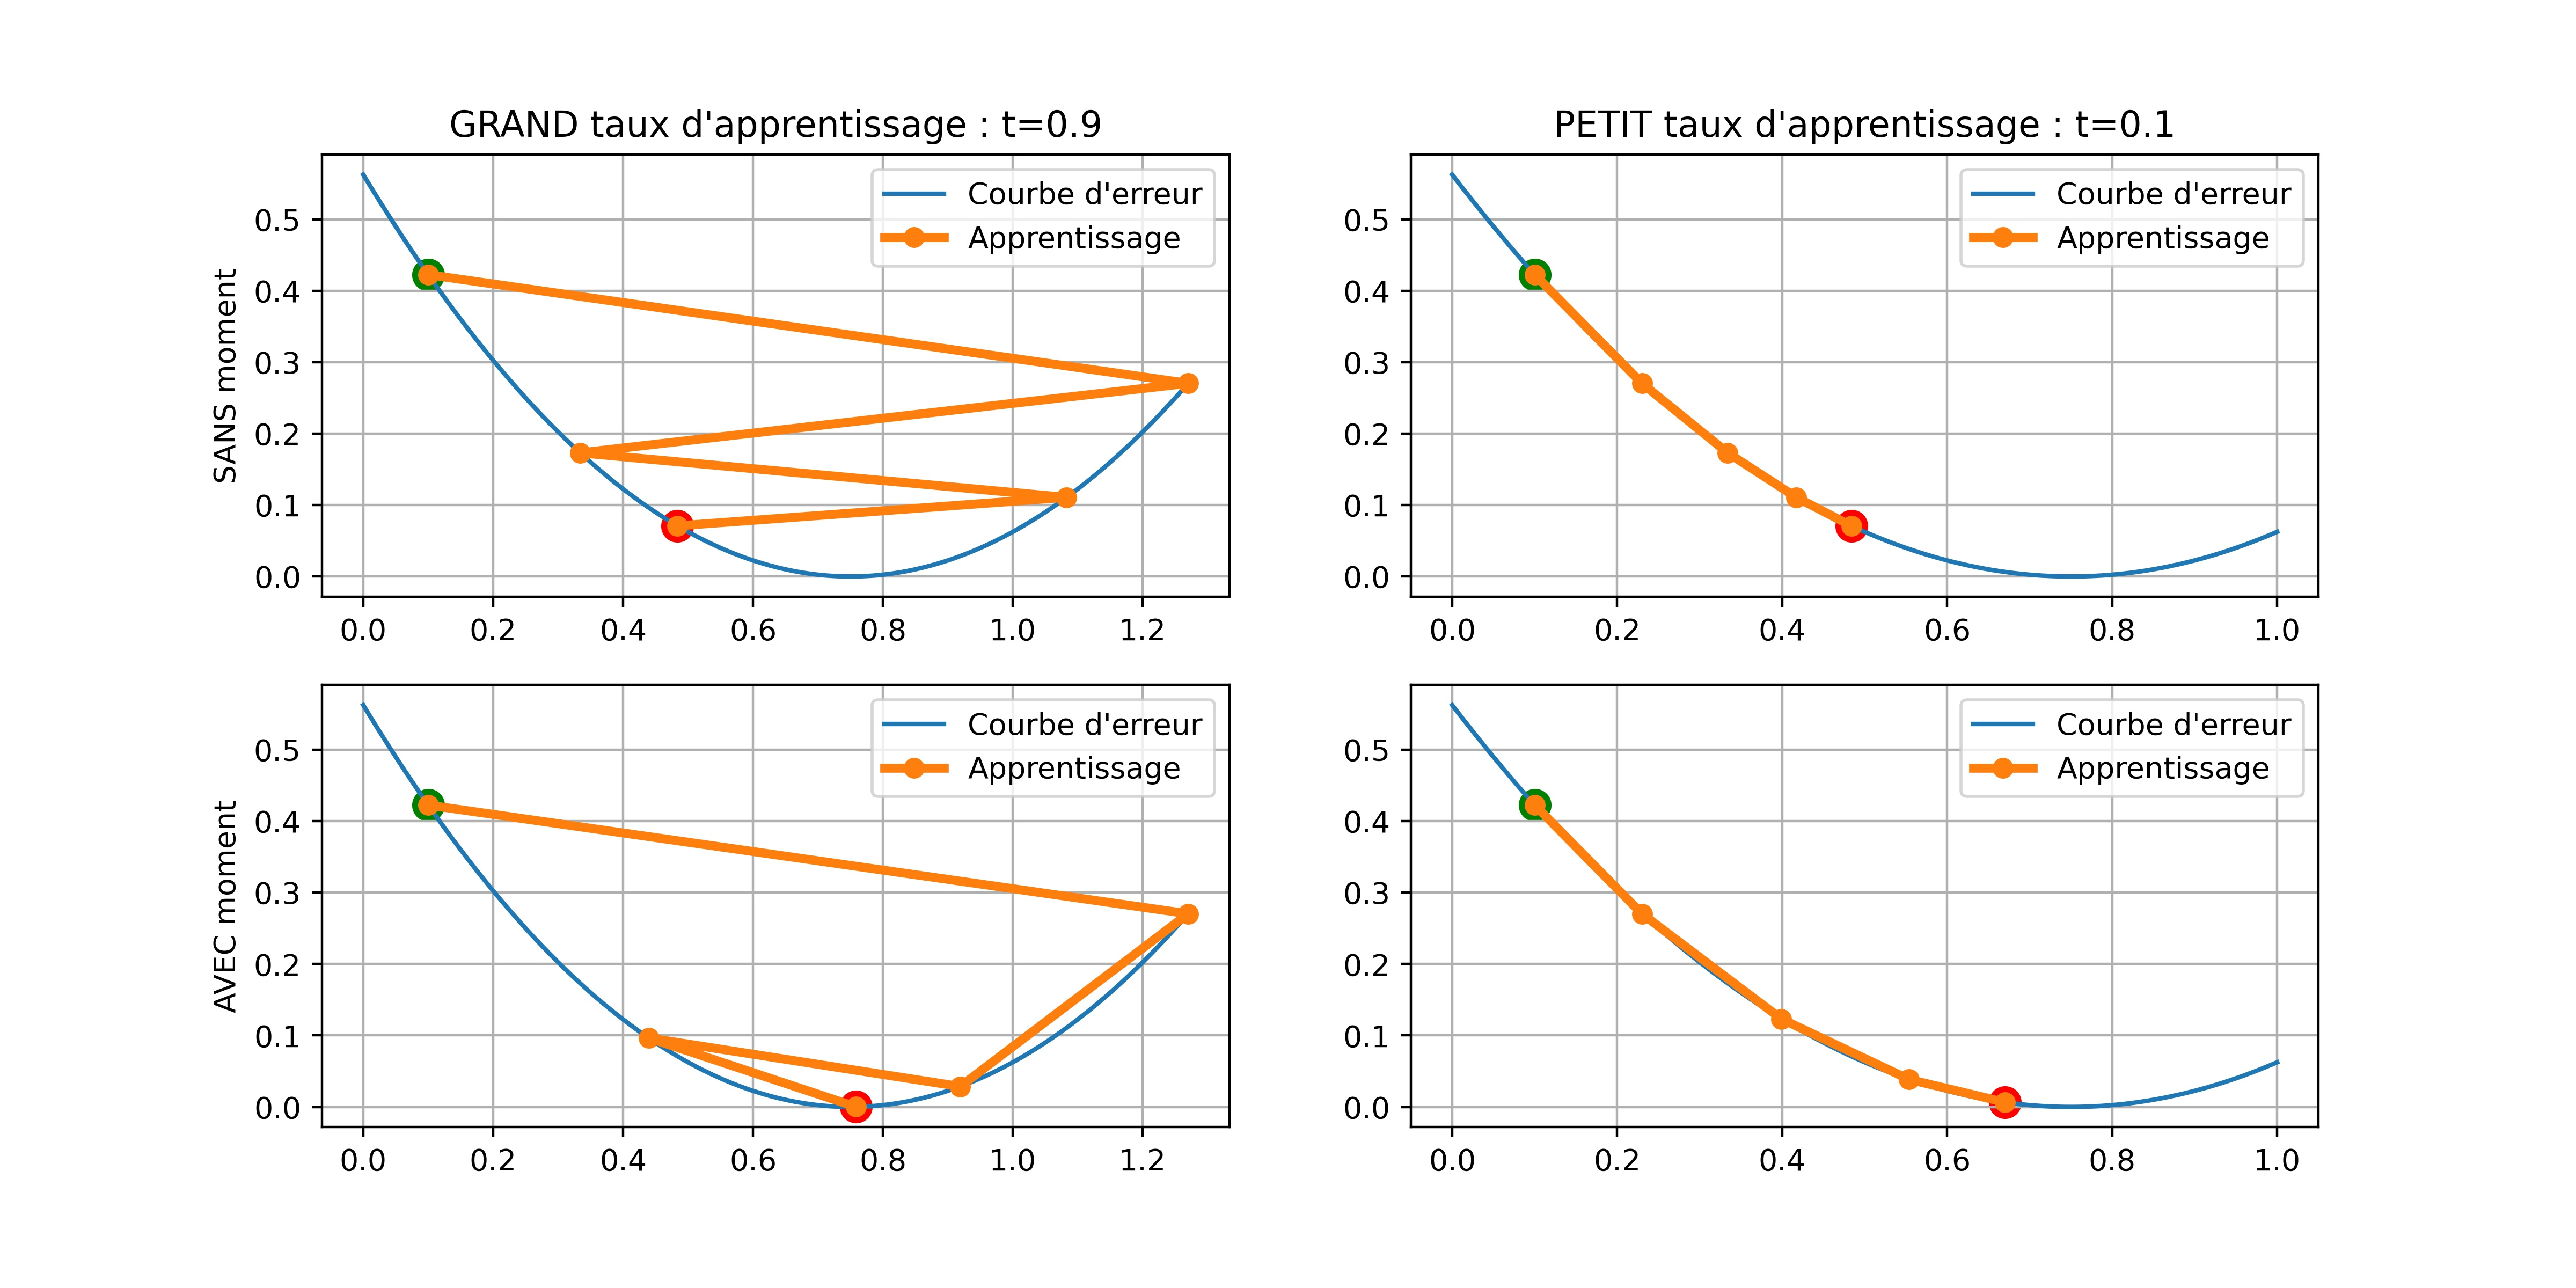
\includegraphics[height=130px, trim=0 35 0 35, clip]{3-Moment.jpg}
        \caption{Descente de gradient SANS/AVEC moment où $\gamma = 0.5$, arrêt à $k=4$}
    \end{figure}
\end{frame}

\begin{frame}{III - Utilisation du Moment}
    Voici, une simulation pour des taux d'apprentissage "trop grand" ou "trop petit".
    \begin{figure}
        \centering
        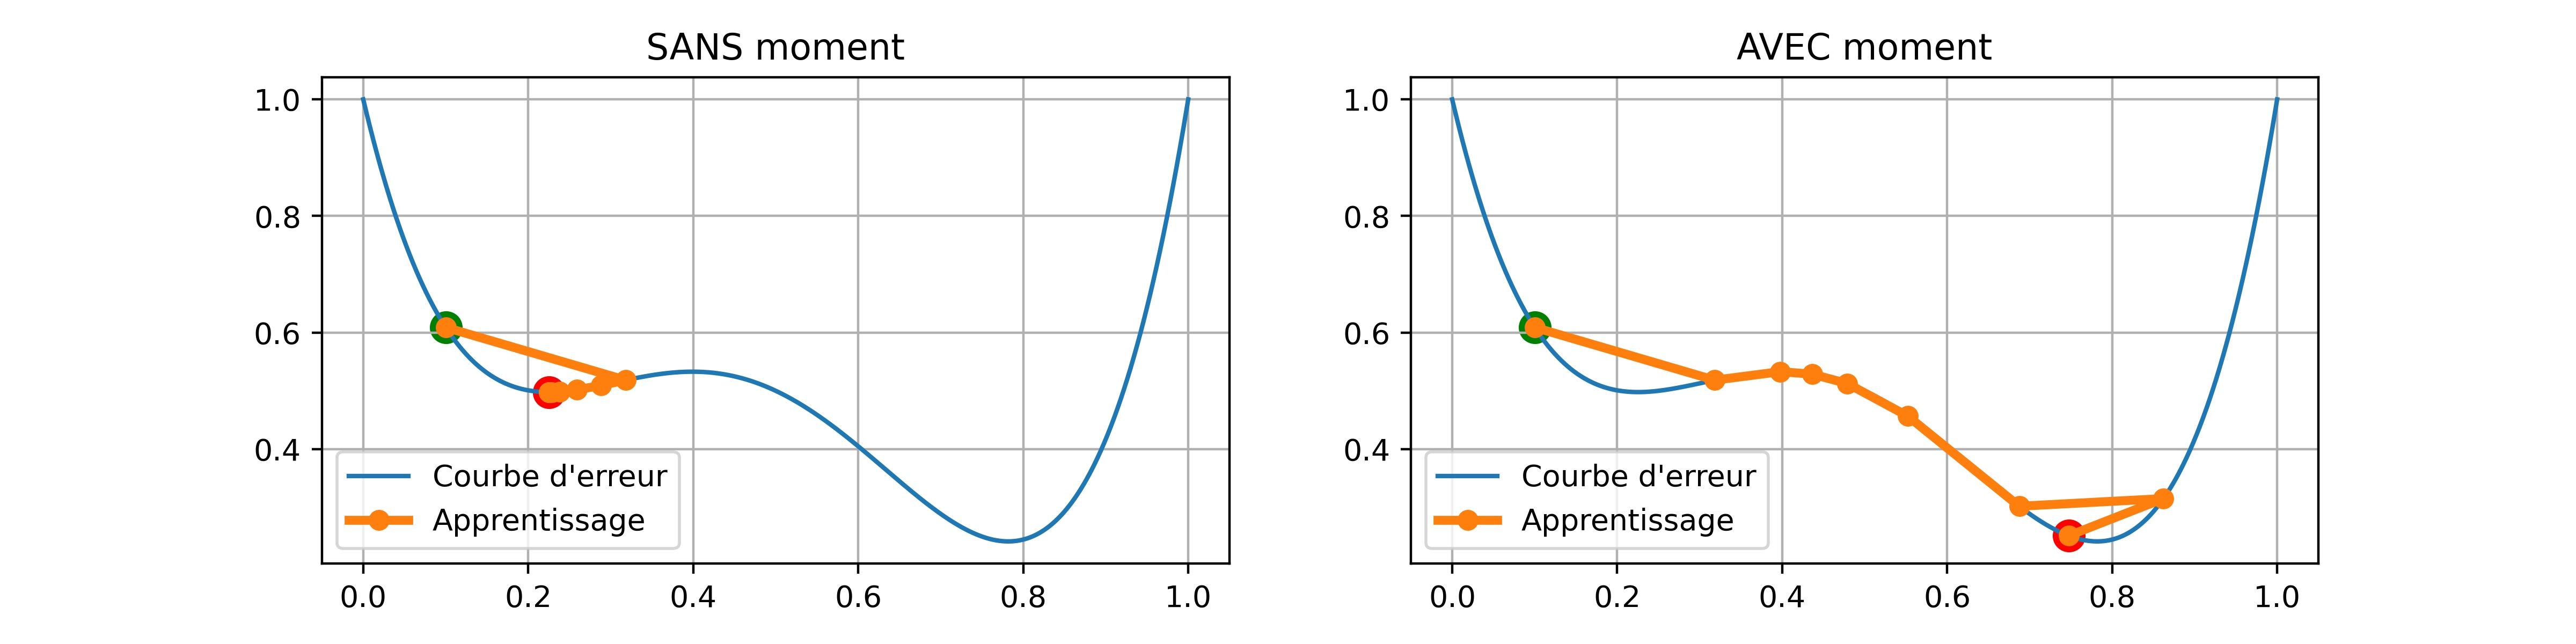
\includegraphics[height=130px, trim=0 35 0 35, clip]{4-Moment.jpg}
        \caption{Descente de gradient SANS/AVEC moment où $\gamma = 0.5$, arrêt à $k=8$}
    \end{figure}
\end{frame}

\begin{frame}{III - Utilisation du Moment}
    Le moment permet également de s'échapper de certains minima locaux.
    \begin{figure}
        \centering
        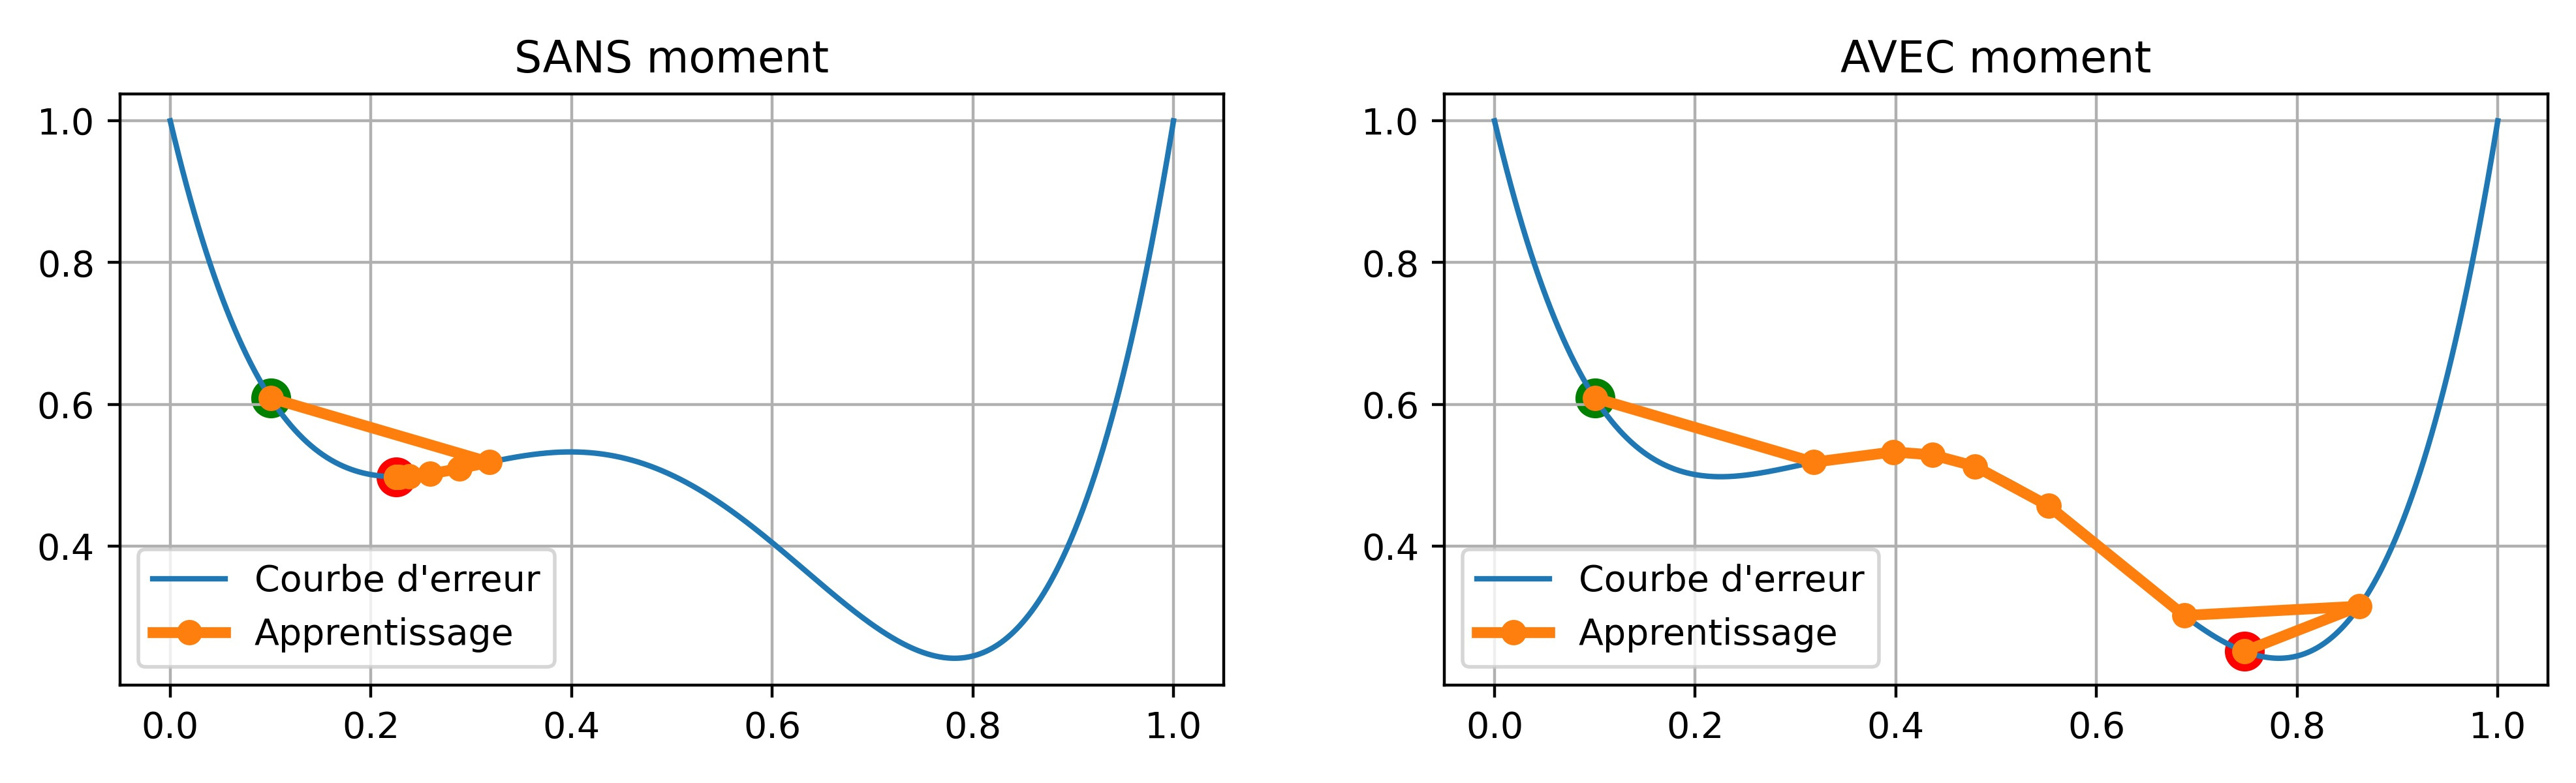
\includegraphics[width=\textwidth, trim=0 10 0 10, clip]{5-Moment.jpg}
        \caption{Descente de gradient SANS/AVEC moment où $\gamma = 0.5$, arrêt à $k=8$}
    \end{figure}
\end{frame}

\begin{frame}{III - Apprentissage stochastique ou par paquet (Batch)}
    Les paramètres du réseau de neurones sont les poids qui pondèrent l'entrée. C'est sur eux que l'on opèrent la descente de gradient. 
    \begin{figure}
        \centering
        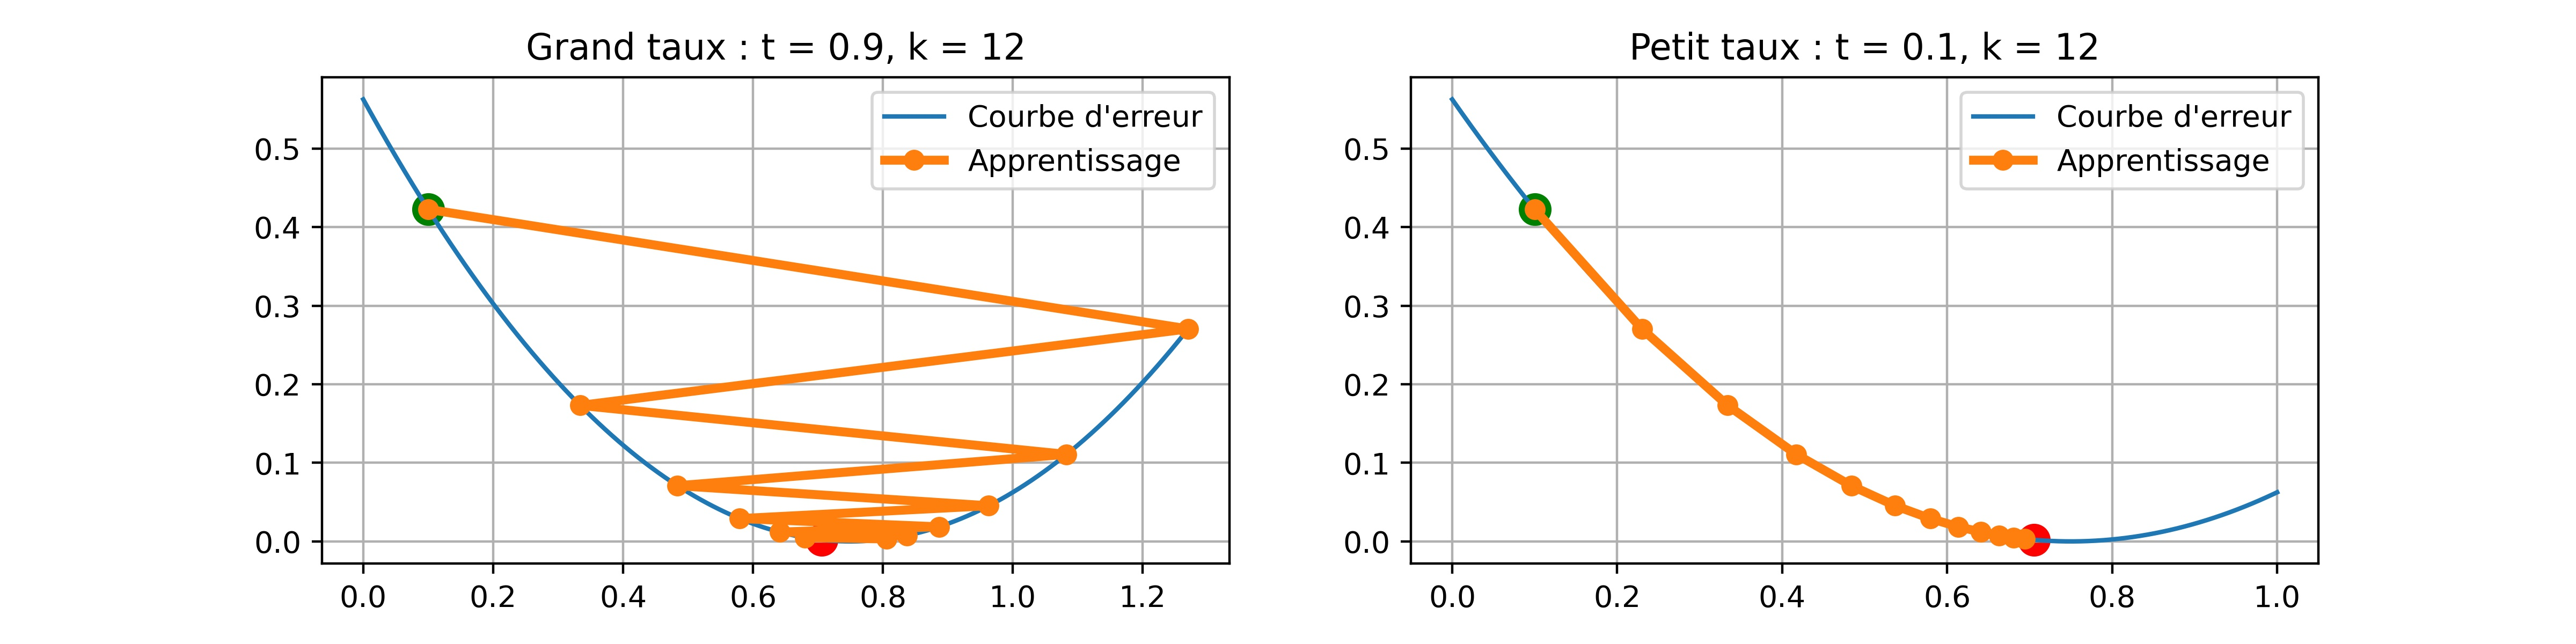
\includegraphics[width=\textwidth]{1-DescenteGradient.jpg}
    \end{figure}
    \begin{figure}
        \centering
        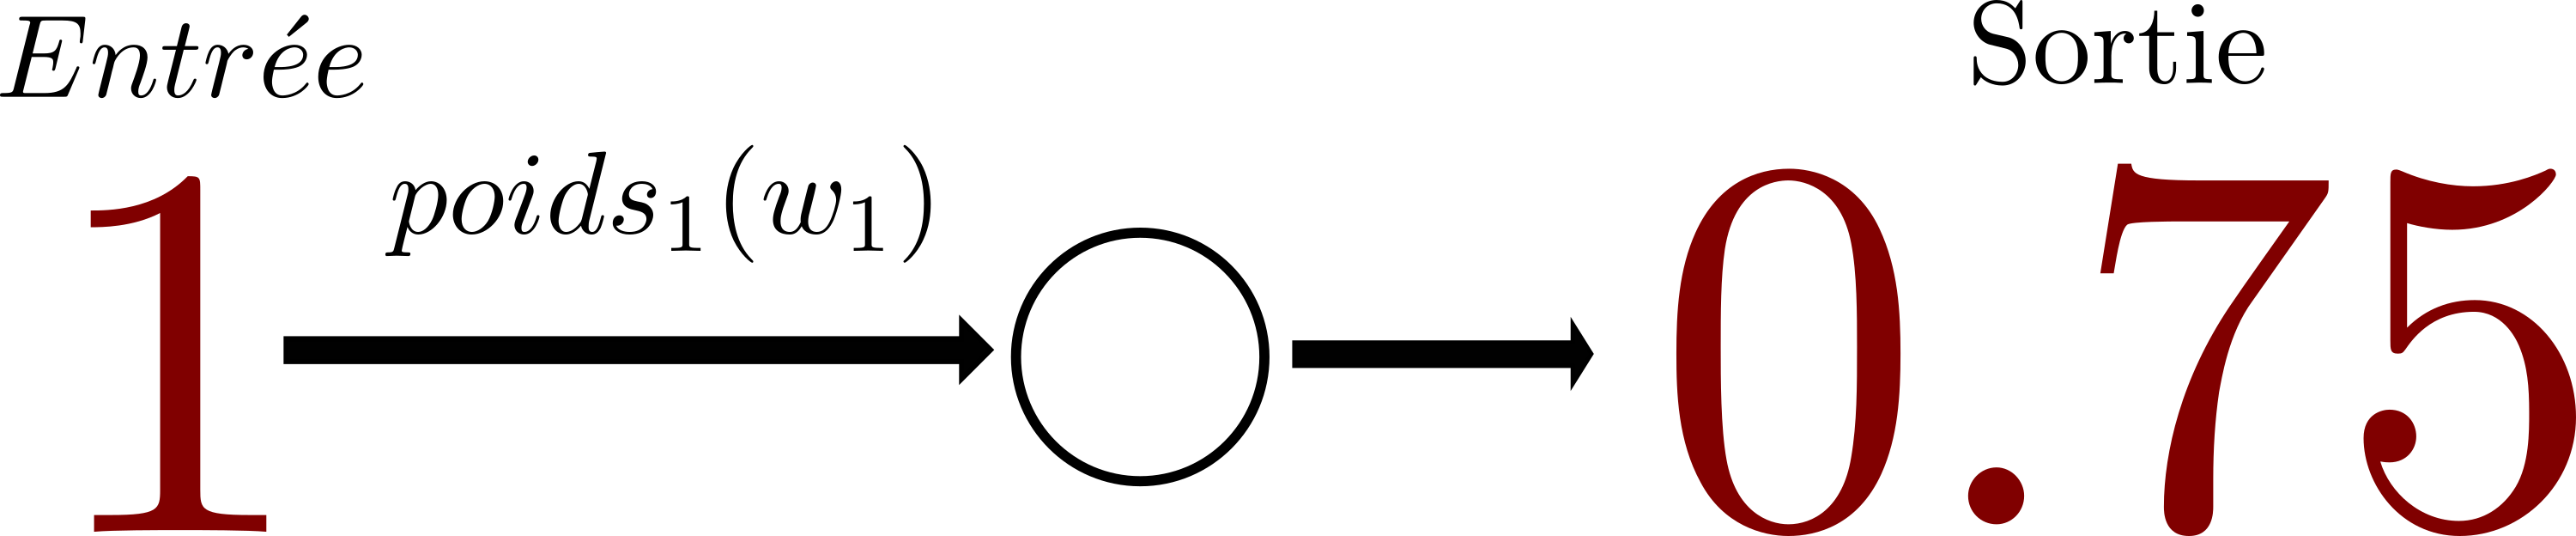
\includegraphics[height=50px]{6-Perceptron.png}
        \caption{Schéma du perceptron linéaire}
    \end{figure}
\end{frame}

\begin{frame}{III - Apprentissage stochastique ou par paquet (Batch)}
    \begin{multicols}{2}
        Il faut prendre en compte le fait que les données d'apprentissage ne sont pas toujours exactes, elles sont forcément inscrites dans une marge d'erreur. 
        \columnbreak
        $
            \left< f
            \left(
            \begin{pmatrix}
                    x_1^{1} & \ldots & x_n^{1} & b      \\
                    \vdots  & \vdots & \vdots  & \vdots \\
                    x_1^{D} & \ldots & x_n^{D} & b
                \end{pmatrix}
            \times
            \begin{pmatrix}
                    w_1    \\
                    \vdots \\
                    w_n    \\
                    w_b
                \end{pmatrix}
            \right) \right>
        $
    \end{multicols}
    \begin{figure}
        \centering
        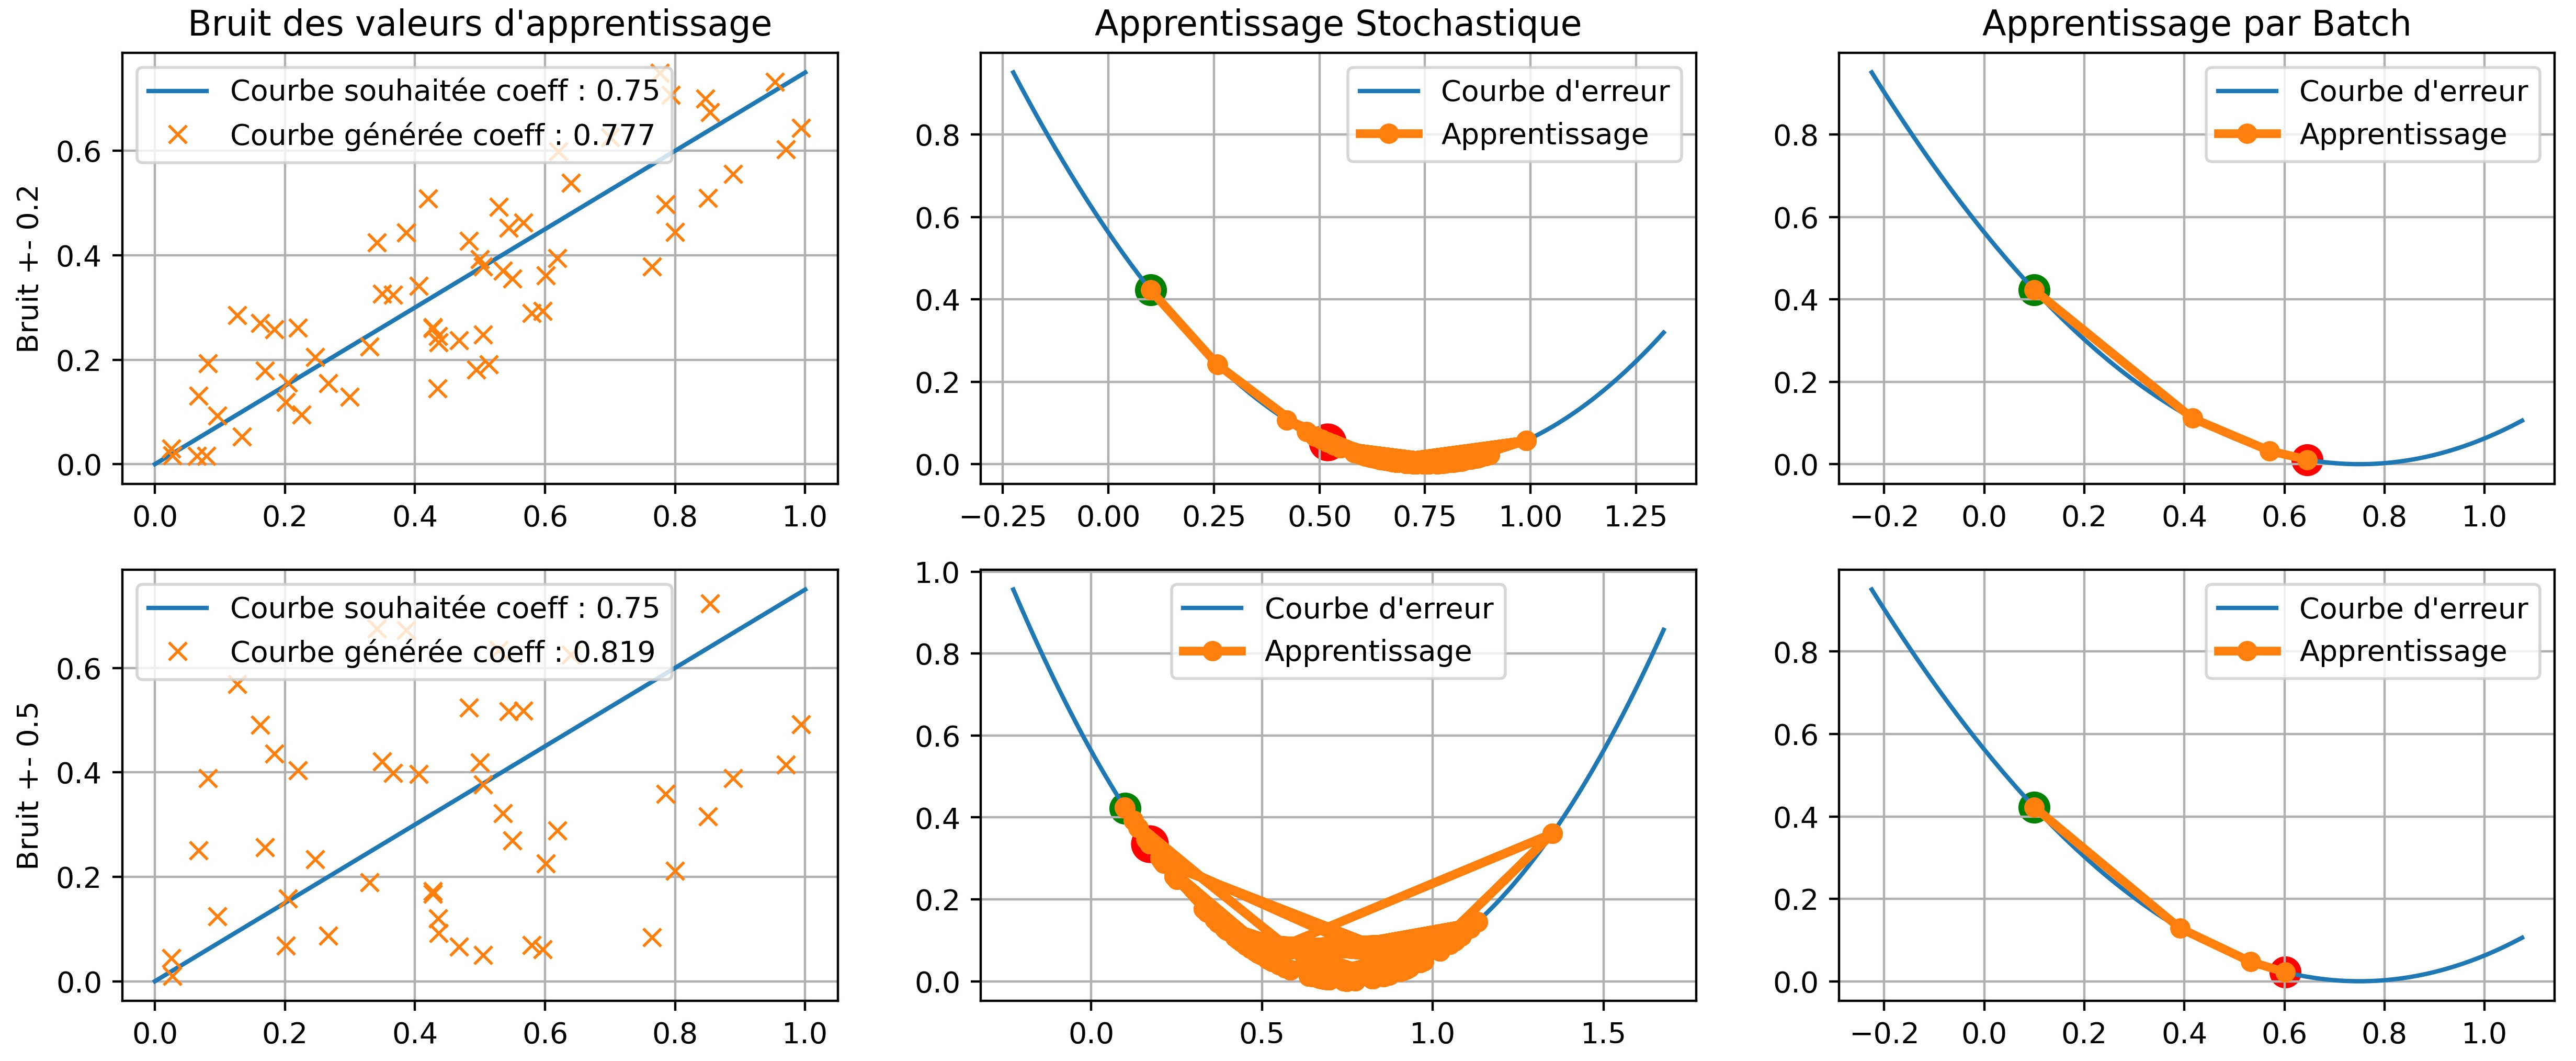
\includegraphics[width=\textwidth, trim=0 30 0 30, clip]{7-Batch.jpg}
        \caption{Comparaison apprentissage stochastique et par paquet, $f(x) = (x-0.75)^2$}
    \end{figure}
\end{frame}
